%================================================================
\chapter{Introduction and Objective of the Study}
%================================================================

%================================================================
\section{Introduction}\label{sec:Introduction}
%================================================================

%================================================================
\subsection{Machine Learning}\label{sec:Machine Learning Intro}
%================================================================


\emph{Machine learning} is the hugely successful field of algorithms that allow computers to solve problems using data, relieving the need for tailoring problem-specific solutions \cite{SupervisedwquantumComputers}. This practice has transformed nearly every aspect of our modern society, from medicine (kilde) to finance (kilde). One of the biggest branches of machine learning is \emph{supervised learning}, which is the practice of training a model to learn a relation between input and output data \cite{hastie01statisticallearning}. Typically, one starts by acquiring a \emph{training set} of \emph{labelled data}, which is a collection of pairs of input and output data. As an example, the inputs and outputs can be \emph{age} and \emph{salary} of people, respectively. By training the a machine learning model on the training set, one hopes that it learns the general relation between \emph{age} and \emph{salary}. If this is the case, the model can be used for predicting the salary of people based on their age, even for values of \emph{age} not present in the training set. If the latter is the case, the model is said to generalize to unseen data, which is required if the model should be used for prediction. How are machine learning models trained? It is typical to define a \emph{loss function} (also commonly known as risk, cost or error function \citet{}), which is a scalar function that measures how accurately a model predicts the outputs from the corresponding inputs \cite{hastie01statisticallearning}. The lower the value of the loss function, the better the model reproduce the outputs. Therefore, training a model involves minimizing the loss function with respect to the training set.

A particular powerful family of machine learning models are the \emph{neural networks} (NN), which are models consisting of layers of artificial neurons, originally inspired by the neural structures in the brain \cite{hands-on}. Neural networks are \emph{parametric} models, meaning that the input-output relation that they compute are determined by a set of real-valued parameters. When setting up a NN, the goal of the training is to find the correct parameters such that the given loss function is minimized. The approach for doing this in practice is to calculate the derivative of the loss function with respect to the parameters of the NN. This derivative is called the \emph{gradient}, and quantifies how the loss function change when the parameters are adjusted. Using gradient-based methods, such as gradient descent, the gradient can be utilized to adjust the parameters loss decreases \cite{hands-on}. The \emph{backpropagation algorithm} is commonly used for calculating the gradient of NNs \cite{hands-on}, tailored for accommodating their layered structure. 

Increasing the number of layers of NNs has been shown to increase their flexibility \cite{raghu2017expressive}, meaning that thay can reproduce the input-output pairs of complex data more easily. However, this comes with a drawback: with increasing number of layers, the \emph{vanishing gradient phenomenon} emerges, meaning the magnitude of the gradient decreases exponentially fast \cite{LeCun2012}. This phenomenon manifests itself as a loss function that is insensitive to adjustments of the parameters, known as a flat \emph{loss landscape}, making the training of many-layered NNs difficult \cite{karakida2019universal}. To uncover the geometry of the loss landscape, and determine its flatness, it is common practice to assess the spectrum of the \emph{empirical fisher information matrix} (EFIM) \cite{karakida2019universal}.


%================================================================
\subsection{Quantum Computing}\label{sec:Quantum Computing Intro}
%================================================================
\emph{Quantum computing} is the study of how information can be processed using systems that obey the laws of quantum mechanics \cite{NielsenQuantum}. In 1982, Richard Feynman pointed out that quantum mechanical systems are notoriously difficult to simulate on classical computers. He suggested that this complexity could be exploited by build a computer based on the principals of quantum mechanics \cite{NielsenQuantum}. Only three years later, David Deutsch formalized a theory describing such a device, a \emph{universal quantum computer} \cite{Deutsch1985QuantumTT}. Even though such a device was not yet realized physically, people started developing algorithms for quantum computers that theorized to be more efficient than their classical counterparts. In 1994, Peter Shor developed Shor's algorithm for factoring integers in polynomial time, which is believed to be exponentially hard on classical computers \cite{Shor_1997}.  

Today, there is a lot of focus on making quantum computers, with big companies such as Google and IBM at the forefront. Despite the effort, today's quantum computers are not able to implement useful quantum algorithms that would change the world right away. This is because today's quantum computers are small and perform very noisy computations \cite{Preskill_2018}. As the quantum computer performs an algorithm, it manipulates a very delicate quantum state. During the span of the computation, the state is susceptible to interference from the surrounding environment, causing the information of the system to degrade. This phenomenon is called \emph{decoherence}, and puts a strict limit on length of the algorithm one can implement \cite{saki2019study}. This makes many of the more promising quantum algorithms, such as Shor's algorithm, unfeasible to implement today.


%================================================================
\subsection{Quantum Machine Learning}\label{sec:Quantum Machine Learning}
%================================================================
By combining machine learning and quantum computing, you get the emerging interdisciplinary field \emph{quantum machine learning}. Just from the name, it is not immediately what it might entail, and as matter of fact, it depends on the context. From \autoref{fig:cccq}, we see the different ways of combining machine learning and quantum computing. In this thesis, we will focus on the CC and CQ combinations. The CC case refers to classical data that is processed on classical devices, which is of course the traditional form of machine learning, e.g. neural networks. The other case, CQ, investigates how classical data can be processed with help of quantum computers.

\begin{figure}[htp]
    \centering
    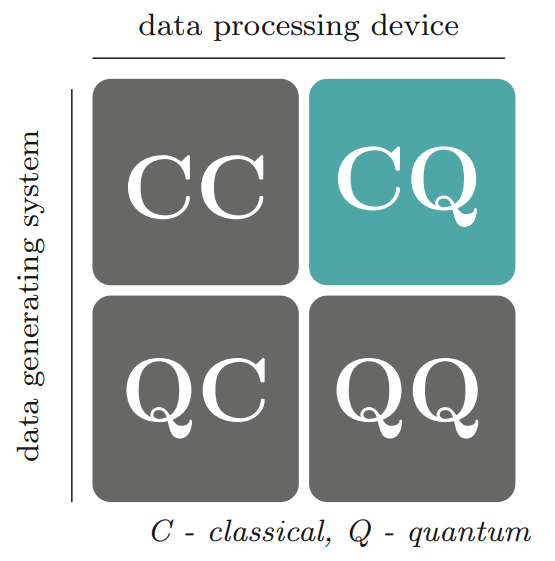
\includegraphics[width=8cm]{latex/figures/cccq.PNG}
    \caption{Four approached that combine machine learning and quantum computing. The figure is retrieved from \citet{SupervisedwquantumComputers}.}
    \label{fig:cccq}
\end{figure}

Lately, there has been many proposals of methods of implementing machine learning using quantum computers. 






Machine learning
\begin{itemize}
    \item Success of machine learning
    \item Neural networks
    \item supervised learning
    \item loss function
    \item gradient -> backpropagation -> vanishing gradient!
    \item manifests as barren plateau -> EFIM
    \item black box -> expressivity -> trajectory length
\end{itemize}

Quantum Computing
\begin{itemize}
    \item Feynman
    \item Superior algorithms -> Shors algorithm
    \item Real hardware -> noisy!
\end{itemize}

Quantum Machine learning
\begin{itemize}
    \item Merging of two disciplines
    \item QQ, QC, CQ, CC
    \item CQ -> using quantum computers for machine learning on classical data
    \item some examples
    \item akin to neural network -> quantum neural network
    \item gradient -> parameter shift rule
    \item bottle-necked by noisy hardware -> few qubits, decoherence, limit the size of the model
    \item also vanishing gradient -> in the number of qubits(and gates)
\end{itemize}

Quantum Circuit Network
\begin{itemize}
    \item Sequential structure of consisting of QNNs
    \item How does one 
    \item Can the use of multiple circuits allow for efficient models with shallow circuits? Will this help the gradient? More easy to estimate gradient? Does the sequential architecture increase the flexibility? Are they possible to train in practice? Suitable for noisy hardware?
\end{itemize}


